% meta.concepts: 2D moment
% meta.tags: realistic
% acknowledge: Peter Seiler & Luke Melander graciously shared Spring 2019 course material
% source: 2019 P. Seiler AEM2011 HW 4


Consider the coordinate system (red lines) attached to the aircraft center of gravity (red dot) depicted in the
diagram below. The positive y-axis, not shown, points into the page (to the right-side of the pilot). The aircraft
weight $W$ acts downward at the center of gravity. The lift $L$ and drag $D$ forces are generated by the airflow
over the wing and act at the center of pressure (black dot) in the negative $z$ and negative $x$ directions,
respectively. The center of pressure is located at $\bar{r}_{CP} = -d {\bf i}$. The engine thrust $T$ is also assumed to act at
the center of pressure in the positive $x$ direction. 

\begin{enumerate}
  \item Assume that all forces balance along the $x$ direction. What lift force $L$ is required to ensure that all forces
  balance along the $z$ direction? Your answer should be expressed in terms of $W$ and $\alpha$. Assume $E = 0$. 
  \item Replace the lift force $L$ computed in the previous part with a force-couple system at the center of gravity.
Your answer should be expressed in terms of $W$ , $\alpha$, and $d$.  Assume $E = 0$.
  \item The tail surface on an aircraft is needed to prevent the aircraft from rotating about the $y$-axis. $E$ is the
  force generated by the flow over the tail surface of the aircraft. This force acts in the negative $z$ direction at $\bar{r}_{E} = -11d{\bf i}$.  What forces $L$ and $E$ are required to ensure that the system is equivalent to zero force and zero moment about the center of gravity?
\end{enumerate}

\begin{figure}[ht!]
  \centering
  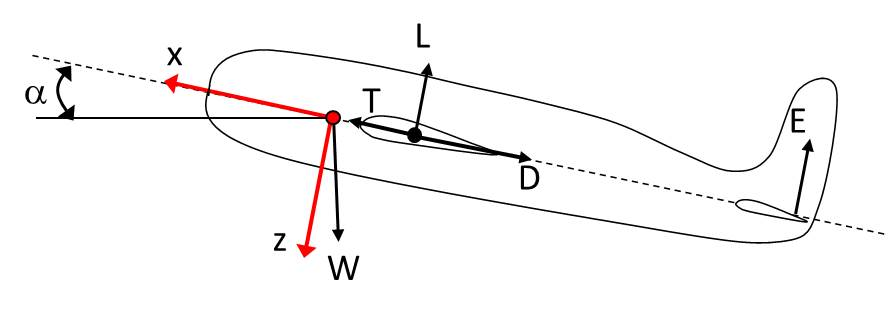
\includegraphics[height=1.8in]{fig.png}
  \caption*{Side-view of aircraft}
\end{figure}

\iftoggle{flagSoln}{%
\vspace{.5cm}
\rule{\textwidth}{.4pt}
\vspace{.5cm}
\textbf{Solution:}
\begin{figure}[ht!]
  \centering
  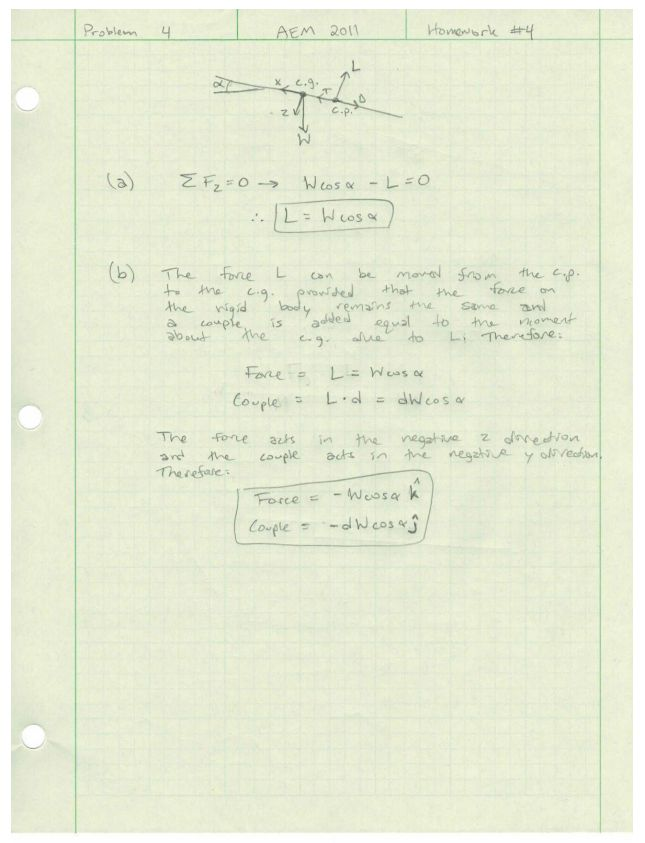
\includegraphics[width=0.45\textwidth,
	           height=0.35\textheight,
		   keepaspectratio]{solna.png}
  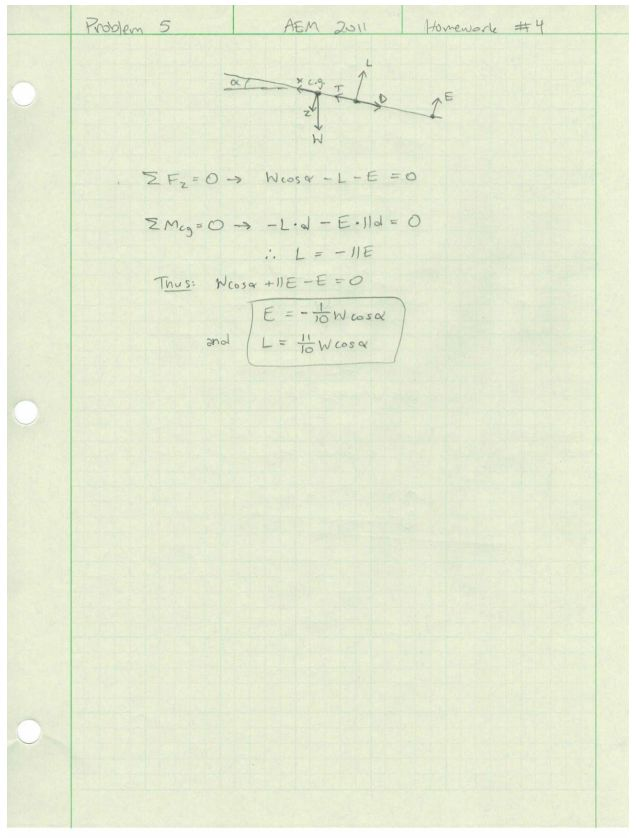
\includegraphics[width=0.45\textwidth,
	           height=0.35\textheight,
		   keepaspectratio]{solnb.png}
\end{figure}
}{%
}%
